\section{Ablation Study}\label{sec:ablation}

To understand which components of the sensing and feature extraction pipeline are critical for classification performance, we conduct a comprehensive ablation study. All ablation experiments use the RF classifier with the raw isolation method (the best-performing configuration without PCA).

\subsection{Sensor Group Ablation}

Table~\ref{tab:sensor_ablation} reports classification accuracy when restricting the feature set to individual sensor groups.

\begin{table}[H]
\caption{Classification accuracy by sensor group. ``All'' uses all 110 sensor channels. Individual Arduino modules use 17 channels each. Electrical uses 8 current sensors.}\label{tab:sensor_ablation}
\centering
\begin{tabular}{lcc}
\toprule
\textbf{Sensor Group} & \textbf{Accuracy (\%)} & \textbf{Features} \\
\midrule
All sensors              & $100.0 \pm 0.0$ & 1{,}540 \\
Arduino (all 6 modules)  & $100.0 \pm 0.0$ & 1{,}428 \\
y\_bed\_\_3              & $100.0 \pm 0.0$ & 238 \\
frame\_l2                & $98.0 \pm 4.0$ & 238 \\
y\_bed\_\_4              & $98.0 \pm 4.0$ & 238 \\
frame\_r2                & $96.0 \pm 4.9$ & 238 \\
spindle2                 & $96.0 \pm 4.9$ & 238 \\
frame\_l3                & $94.0 \pm 8.0$ & 238 \\
Electrical (current only) & $76.5 \pm 12.4$ & 112 \\
\bottomrule
\end{tabular}
\end{table}

The y\_bed\_\_3 sensor module alone achieves 100\% accuracy with only 238 features, demonstrating that a single well-placed IMU on the machine bed is sufficient for perfect toolpath classification. This finding has practical significance: a minimal sensor deployment of one IMU near the workpiece can match the performance of the full 10-sensor array. The electrical current sensors alone achieve only 76.5\% accuracy (112 features; corrected from an earlier leaked figure of 96.0\%/350 features that had folded IMU channels into the electrical set, Section~\ref{sec:results}), confirming that motor-current monitoring is substantially less discriminative than vibration sensing on this task---consistent with the near-constant spindle current under the shallow UHMW-PE cut.

\subsection{Feature Statistic Ablation}

Table~\ref{tab:stat_ablation} examines how many summary statistics per temporal bin are needed.

\begin{table}[H]
\caption{Classification accuracy as a function of the number of summary statistics computed per temporal bin.}\label{tab:stat_ablation}
\centering
\begin{tabular}{lcc}
\toprule
\textbf{Statistic Set} & \textbf{Accuracy (\%)} & \textbf{Features} \\
\midrule
Mean + RMS (2 stats)             & $98.0 \pm 4.0$ & 440 \\
Mean + RMS + Std (3 stats)       & $98.0 \pm 4.0$ & 660 \\
All 7 statistics                 & $100.0 \pm 0.0$ & 1{,}540 \\
\bottomrule
\end{tabular}
\end{table}

Even with only two statistics (mean and RMS), classification accuracy reaches 98\%, indicating that the temporal bin means and RMS values capture most of the discriminative information. The full 7-statistic set adds higher-order statistics (skewness, kurtosis) that contribute the final 2\% improvement.

\subsection{Alignment Ablation: Temporal Binning vs.\ Whole-Run Summary}

Table~\ref{tab:alignment_ablation} compares the temporal binning approach against whole-run summary statistics.

\begin{table}[H]
\caption{Classification accuracy for temporal binning ($B = 20$, aggregated to mean + std across bins) vs.\ whole-run summary statistics (no temporal structure).}\label{tab:alignment_ablation}
\centering
\begin{tabular}{lcc}
\toprule
\textbf{Approach} & \textbf{Accuracy (\%)} & \textbf{Features} \\
\midrule
Temporal binning (20 bins)  & $100.0 \pm 0.0$ & 1{,}540 \\
Whole-run summary           & $98.0 \pm 4.0$ & 770 \\
\bottomrule
\end{tabular}
\end{table}

Temporal binning outperforms whole-run summary by 2 percentage points. While modest, this confirms that the temporal evolution of sensor statistics carries discriminative information. The temporal approach also enables the fingerprint visualizations (Figure~\ref{fig:fingerprint}) that provide interpretable insight into how toolpath types differ.

\subsection{PCA Ablation}

Table~\ref{tab:pca_ablation} examines the effect of PCA dimensionality reduction across all three classifiers.

\begin{table}[H]
\caption{Classification accuracy (\%) vs.\ PCA component count, for all three classifiers with raw features. RF shows invariance to component count (all reduce to 88.2\%), while SVM and MLP exhibit different sensitivity patterns.}\label{tab:pca_ablation}
\centering
\begin{tabular}{lccc}
\toprule
\textbf{Components} & \textbf{RF} & \textbf{SVM} & \textbf{MLP} \\
\midrule
No PCA (1{,}540)  & $100.0 \pm 0.0$ & $90.0 \pm 6.3$ & $86.0 \pm 10.2$ \\
2                  & $90.2 \pm 0.4$ & $90.2 \pm 0.4$ & $58.9 \pm 2.2$ \\
3                  & $88.2 \pm 4.1$ & $90.2 \pm 6.3$ & $74.2 \pm 12.2$ \\
5                  & $88.2 \pm 4.1$ & $94.0 \pm 4.9$ & $76.2 \pm 10.5$ \\
10                 & $88.2 \pm 4.1$ & $92.0 \pm 7.5$ & $90.0 \pm 12.6$ \\
15                 & $88.2 \pm 4.1$ & $92.0 \pm 7.5$ & $92.0 \pm 7.5$ \\
20                 & $88.2 \pm 4.1$ & $92.0 \pm 7.5$ & $88.2 \pm 4.1$ \\
30                 & $88.2 \pm 4.1$ & $92.0 \pm 7.5$ & $80.5 \pm 13.8$ \\
\bottomrule
\end{tabular}
\end{table}

The PCA results reveal classifier-dependent behavior. RF accuracy drops to exactly 88.2\% for any number of PCA components from 3 to 30, because the leading principal components contain sufficient class-separating variance for the RF decision boundaries, and additional components add only noise within the PCA-reduced space. In contrast, SVM accuracy \textit{improves} with PCA to 5 components (94.0\%), likely because PCA removes irrelevant high-dimensional noise that the RBF kernel is sensitive to. MLP shows non-monotonic behavior, peaking at 15 components (92.0\%) before degrading due to overfitting in higher dimensions with only 51 training samples. These results demonstrate that dimensionality reduction interacts strongly with classifier choice, and that the ``PCA hurts RF'' finding should not be generalized to all classifiers.

\textbf{PCA misclassification analysis.} To explain why RF accuracy is invariant to PCA component count, we examined which individual samples are misclassified across all PCA configurations. The same 5--6 samples are misclassified in \textit{every} PCA setting (3 through 30 components): pocket150025\_001, pocket150025\_002, pocket150025\_012, face150025\_001, face150025\_010, and (in most settings) pocket150025\_006. These runs are consistently confused between the pocketing and facing classes. This confirms that the invariance is not a statistical artifact but reflects a genuine decision boundary: PCA projects the data into a subspace where these specific runs fall near the class boundary, and no amount of additional PCA dimensions resolves the ambiguity. Without PCA, the full 1{,}540-dimensional feature space provides sufficient redundancy for RF to correctly classify these borderline runs.

\subsection{Learning Curve}

Figure~\ref{fig:learning_curve} shows classification accuracy as a function of training set size.

\begin{figure}[H]
    \centering
    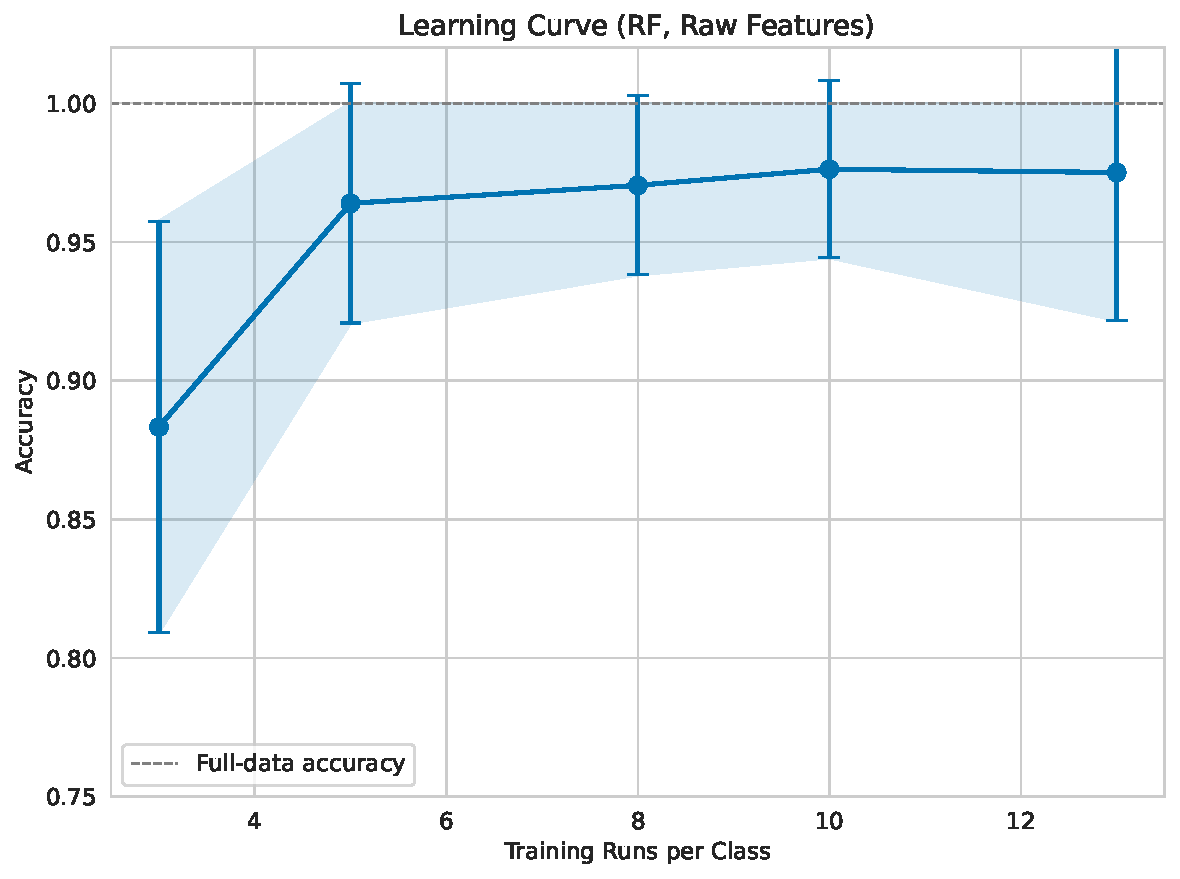
\includegraphics[width=0.7\textwidth]{figures/fig8_learning_curve.pdf}
    \caption{Learning curve: classification accuracy vs.\ number of training runs per class, using RF with raw features. Results are averaged over 10 random subsampling repeats.}
    \label{fig:learning_curve}
\end{figure}

With only 5 training runs per class (15 total), the classifier achieves 96.4\% accuracy. Performance plateaus above 8 runs per class at approximately 97\%. This steep learning curve demonstrates that the toolpath fingerprints are highly distinctive, requiring minimal training data.

\subsection{Sensor Contribution Heatmap}

Figure~\ref{fig:sensor_heatmap} provides a comprehensive view of how each sensor group performs across all four isolation methods.

\begin{figure}[H]
    \centering
    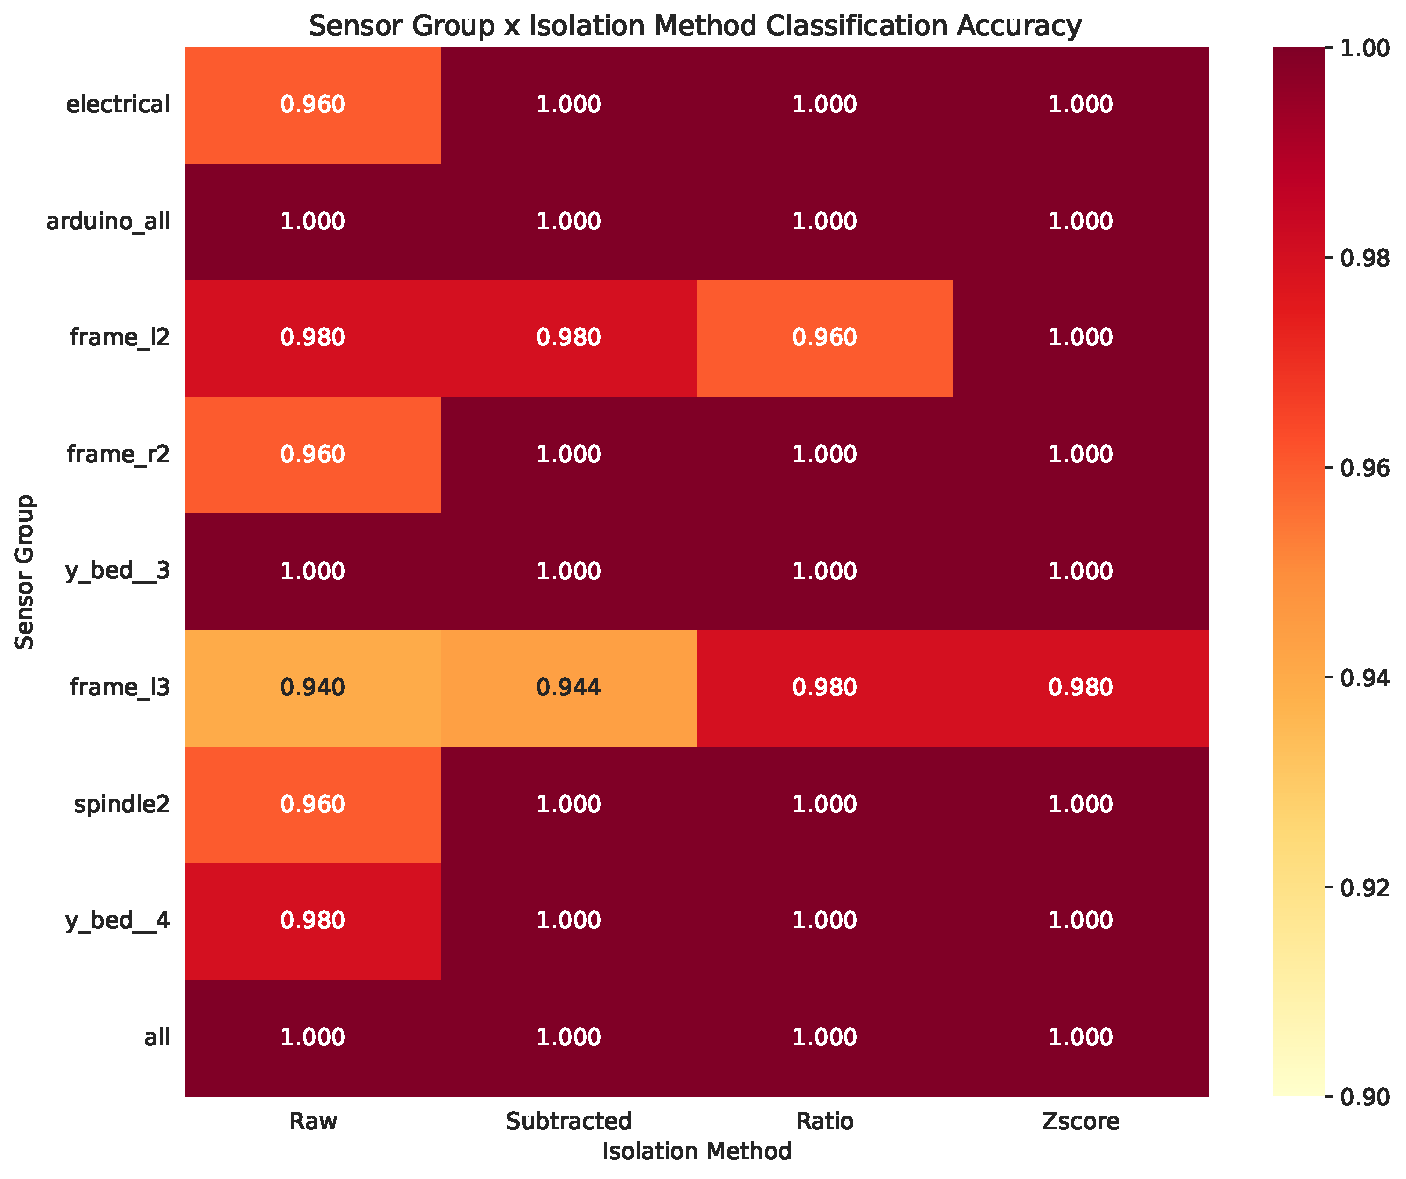
\includegraphics[width=0.85\textwidth]{figures/fig9_sensor_heatmap.pdf}
    \caption{Classification accuracy heatmap by sensor group (rows) and isolation method (columns), using the RF classifier. Darker colors indicate higher accuracy.}
    \label{fig:sensor_heatmap}
\end{figure}

The heatmap reveals that sensor performance is relatively consistent across isolation methods, suggesting that the sensor placement (physical position on the machine) is more important than the signal normalization strategy for this classification task.

\subsection{Noise Robustness}

To assess how sensitive each isolation method is to measurement noise, we add zero-mean Gaussian noise scaled by increasing fractions of the per-feature standard deviation and measure classification accuracy (Figure~\ref{fig:noise_robustness}).

\begin{figure}[H]
    \centering
    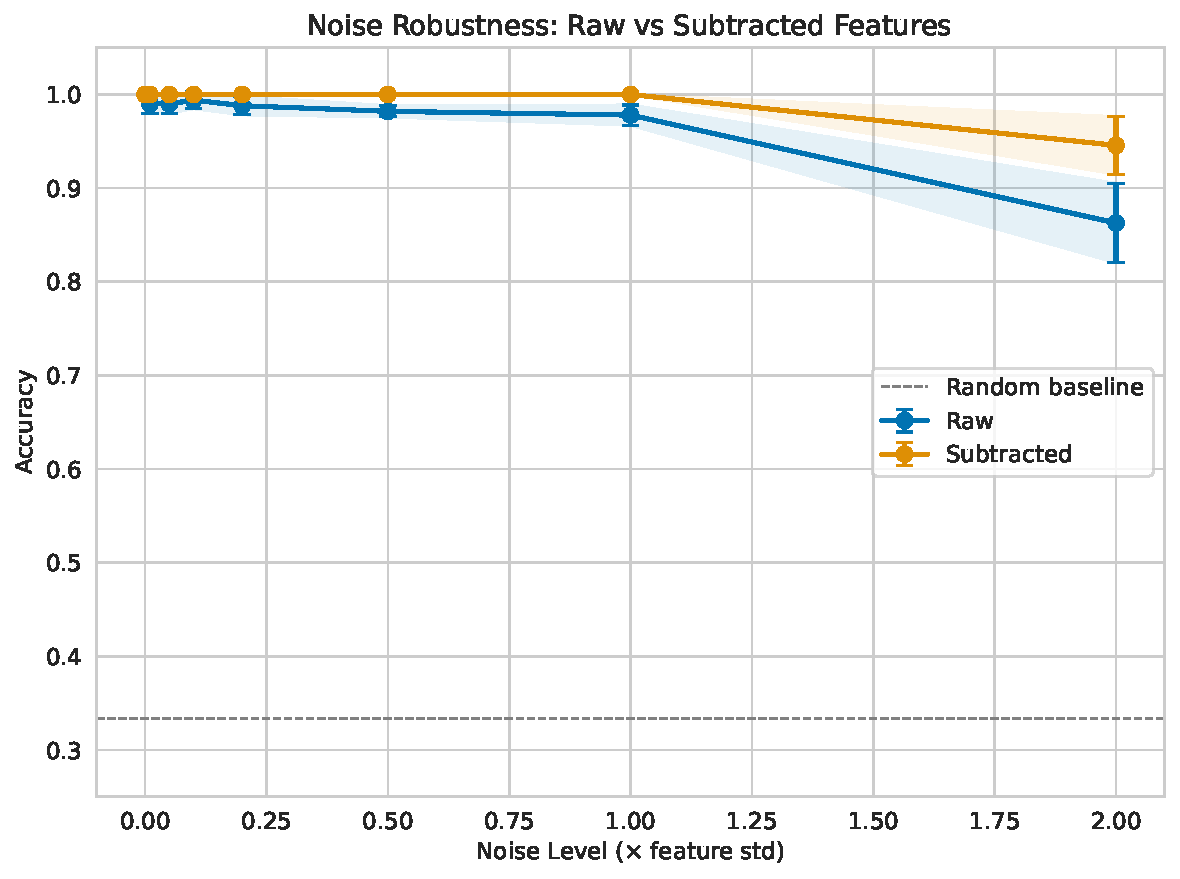
\includegraphics[width=0.7\textwidth]{figures/fig10_noise_robustness.pdf}
    \caption{Noise robustness: classification accuracy vs.\ additive Gaussian noise level (as a fraction of per-feature standard deviation). Subtracted features maintain 100\% accuracy up to $1.0\times$ noise, while raw features degrade to 97.8\%.}
    \label{fig:noise_robustness}
\end{figure}

Subtracted features are dramatically more noise-robust than raw features: they maintain 100\% accuracy up to $1.0\times$ noise (where the added noise equals the feature's natural standard deviation), while raw features degrade to 97.8\% at the same level. At $2.0\times$ noise, subtracted features still achieve 94.6\% vs.\ 86.3\% for raw. This result provides the strongest practical argument for air-cut referencing: the referenced features are substantially more resilient to sensor degradation, calibration drift, and environmental interference.

\subsection{Temporal Bin Importance}

Figure~\ref{fig:bin_importance} shows the accuracy impact of removing each of the 20 temporal bins.

\begin{figure}[H]
    \centering
    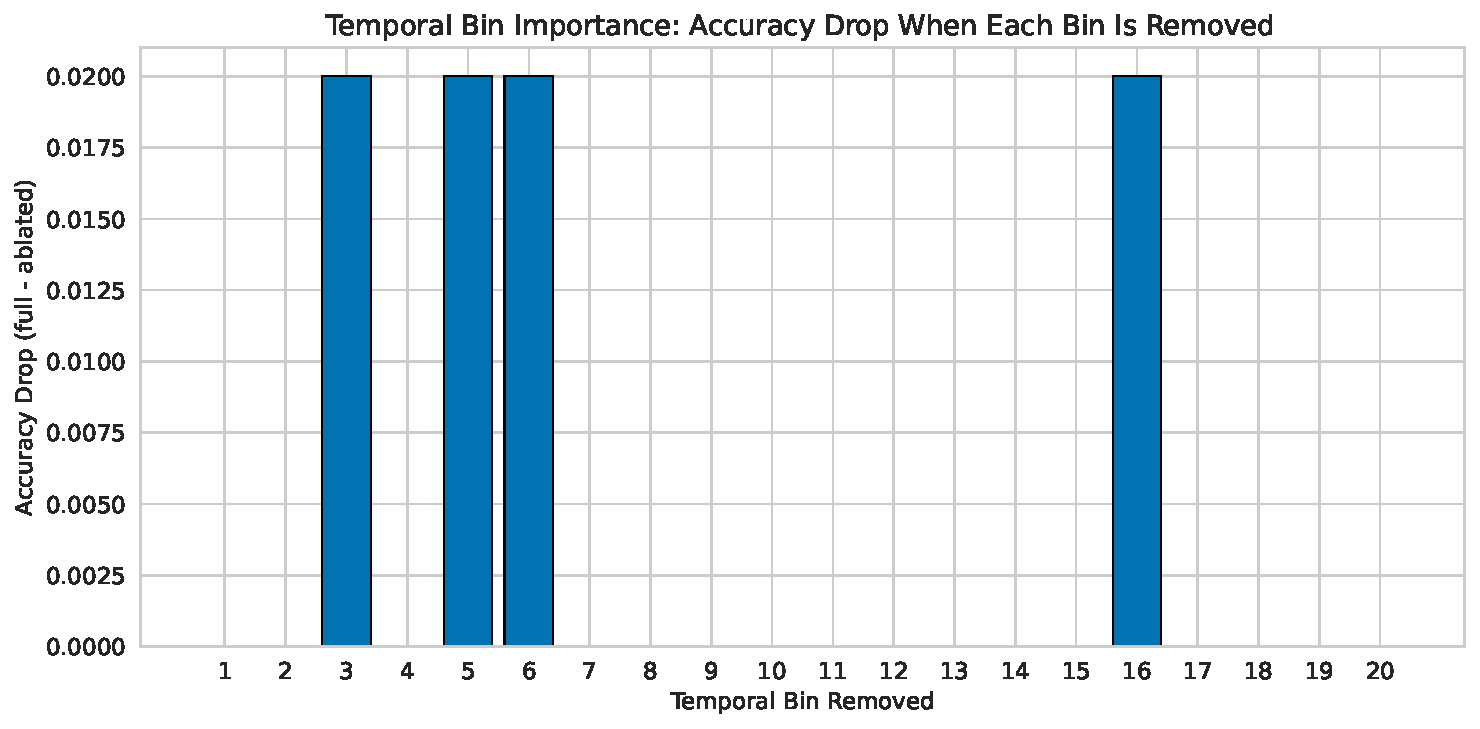
\includegraphics[width=0.85\textwidth]{figures/fig11_bin_importance.pdf}
    \caption{Accuracy drop when each temporal bin is removed (full accuracy minus leave-one-bin-out accuracy). Positive values indicate bins that contribute to classification. Bins 3, 5, 6, and 16 contribute most (each a 2-pp accuracy drop when removed).}
    \label{fig:bin_importance}
\end{figure}

Four bins share the largest impact: bins 3, 5, 6, and 16 (1-indexed), each causing a 2 percentage point drop to 98.0\% when removed. These correspond to approximately 10--30\% of normalized program time (the approach and early cutting phases) and 75--80\% (late cutting phase). The remaining 16 bins can each be removed without any accuracy loss, confirming that the temporal fingerprint's discriminative power is concentrated in specific program phases rather than distributed uniformly across the execution. This finding has practical implications: a coarser binning strategy focused on these critical phases could achieve comparable accuracy with fewer features.

Figure~\ref{fig:ablation_summary} summarizes the core ablation results in a composite figure.

\begin{figure}[H]
    \centering
    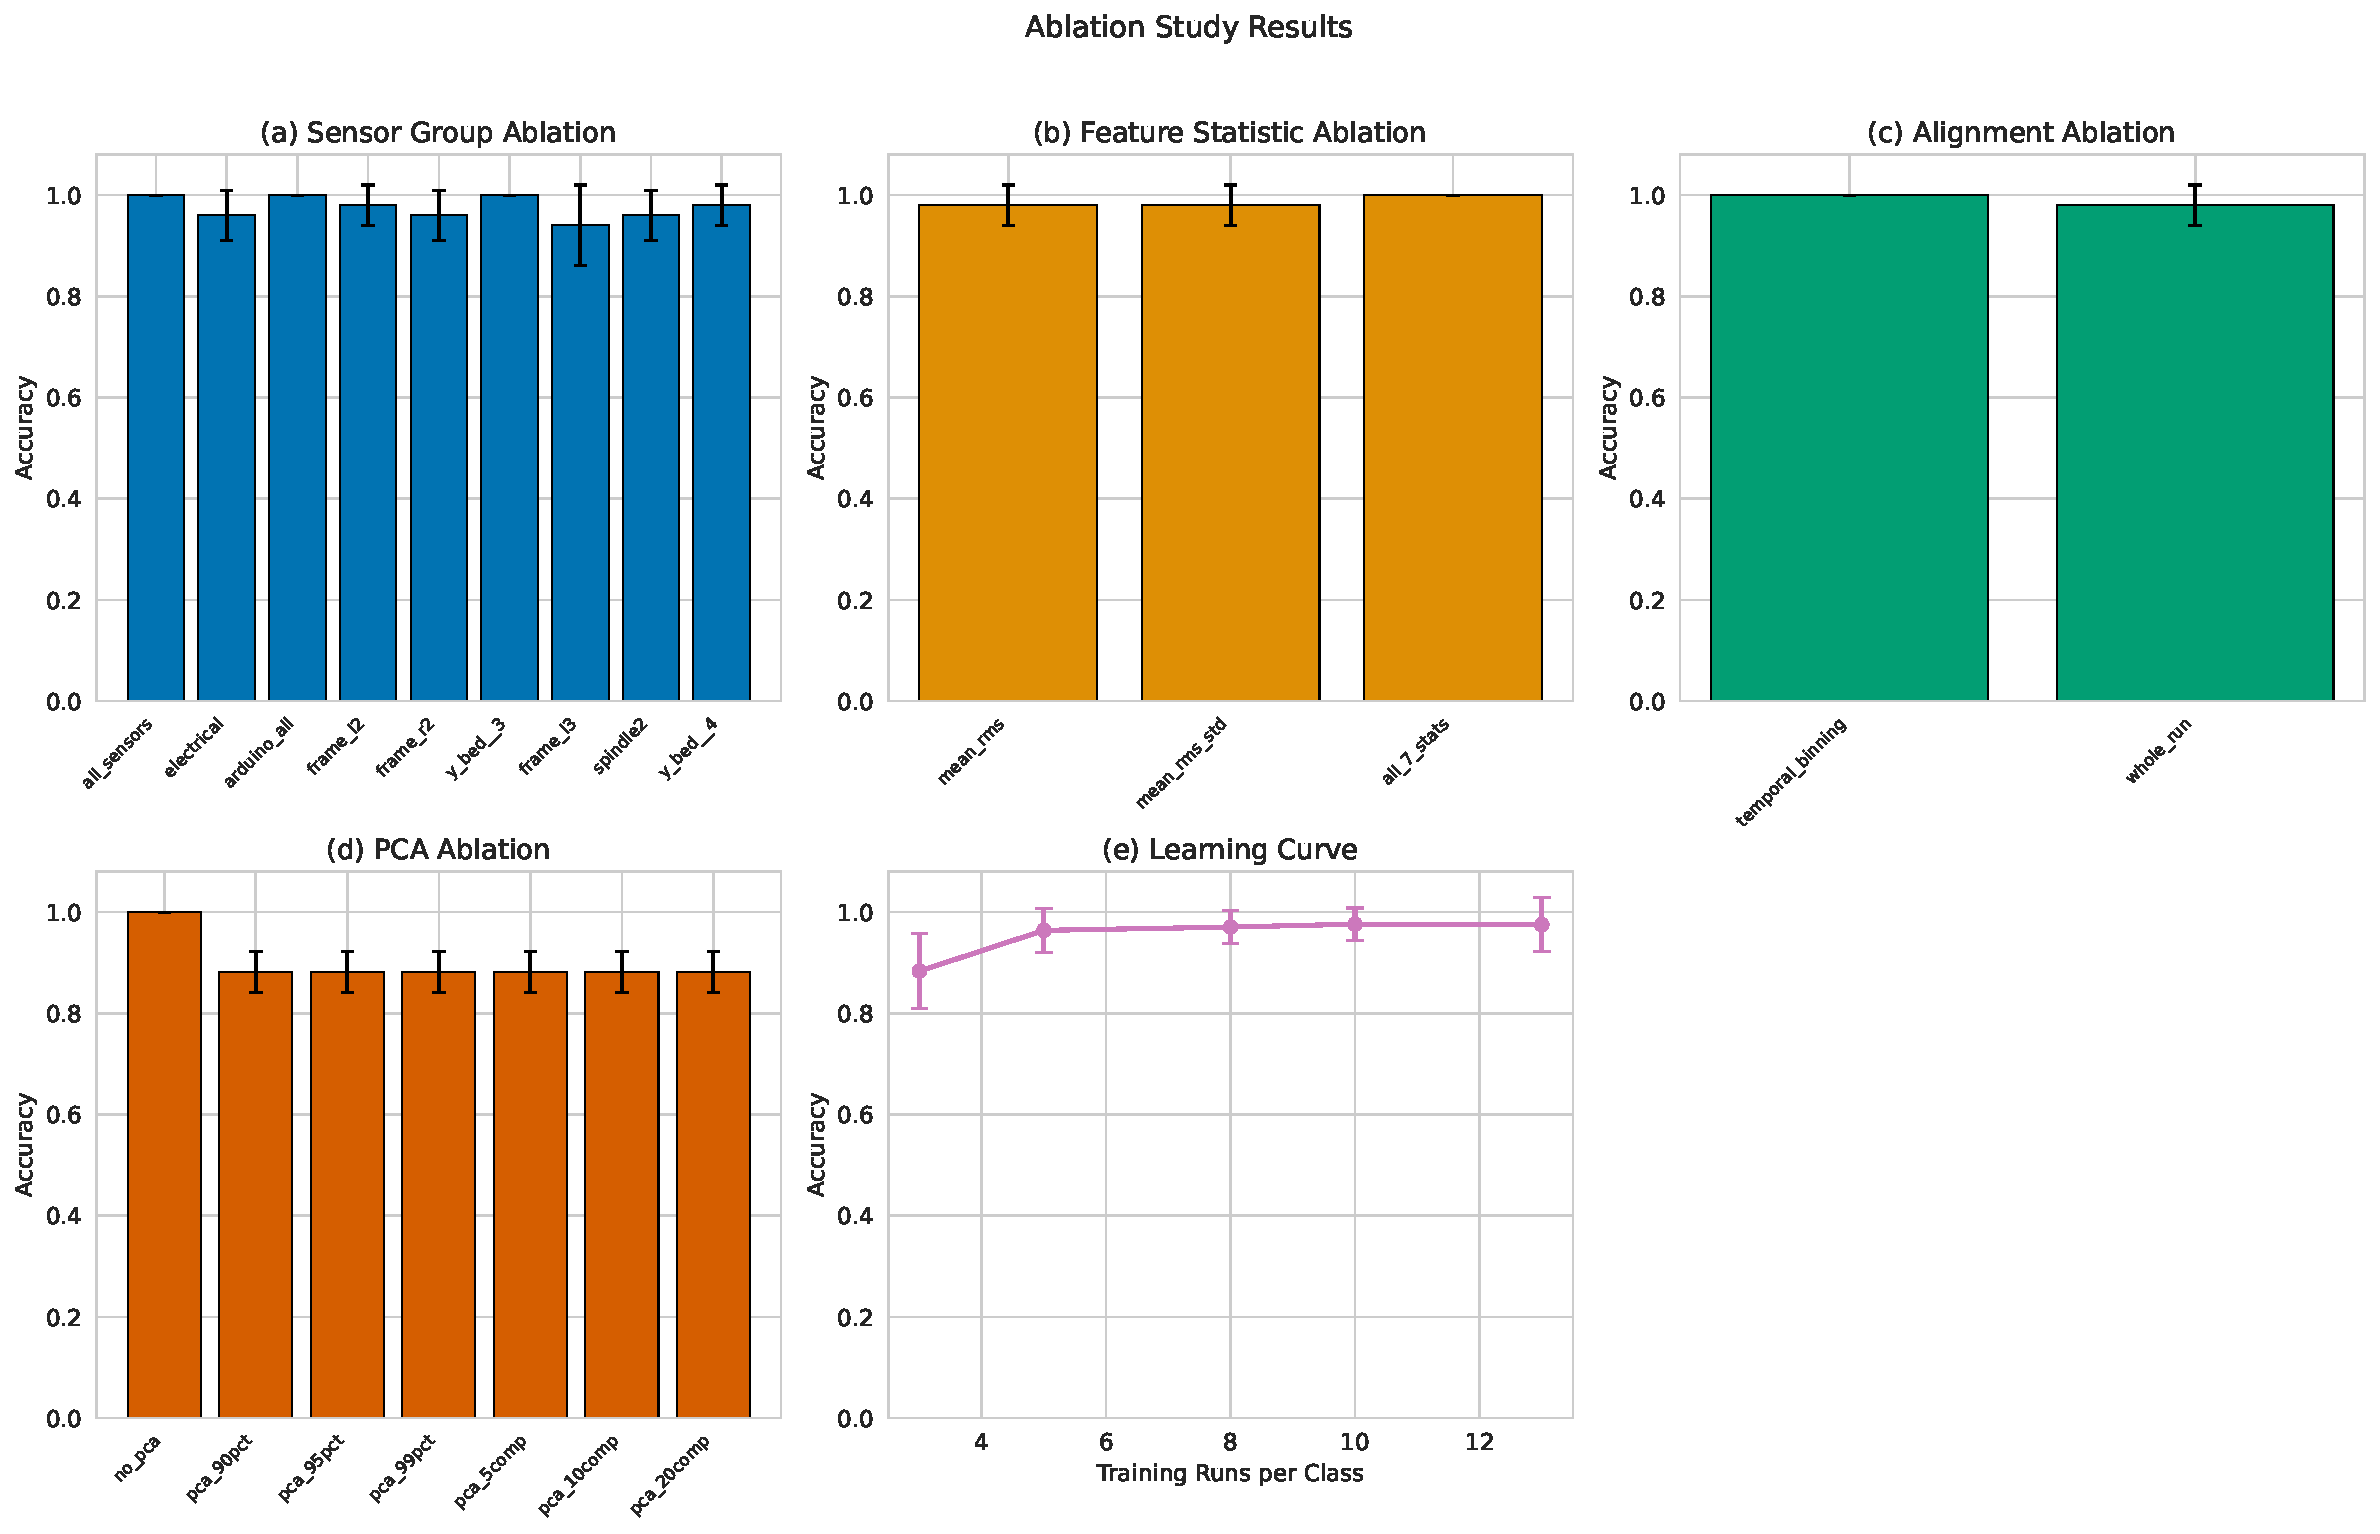
\includegraphics[width=\textwidth]{figures/fig7_ablation.pdf}
    \caption{Summary of core ablation studies: (a)~sensor group, (b)~feature statistics, (c)~alignment method, (d)~PCA configuration, (e)~learning curve.}
    \label{fig:ablation_summary}
\end{figure}
